\author{Kővári Bence}
\neptunCode{IFWY0R}
\courseName{Adatbázis és big data technológiák}
\documentumTypeName{Feladat dokumentáció}

\title{Csatlakozási lehetőségek tesztelése}

\section{Csatlakozási lehetőségek}
\subsection{Oracle Cloud Services Oracle adatbázis}
Szeretnék az Oracle Cloud Services (OCI)-n belül létrehozni egy Oracle adatbázist, és azt csatlakoztatni a vizualizációs eszközhöz. Ennek érdekében regisztráltam egy trial accountot, és létrehoztam egy Oracle Database Instance-t. Az adatbázis egy Standard Edition 12.2-es verziójú. Ezt követően a új kapcsolatot hoztam létre a csatlakozás érdekében:
\begin{figure}[h!]
	\centering
	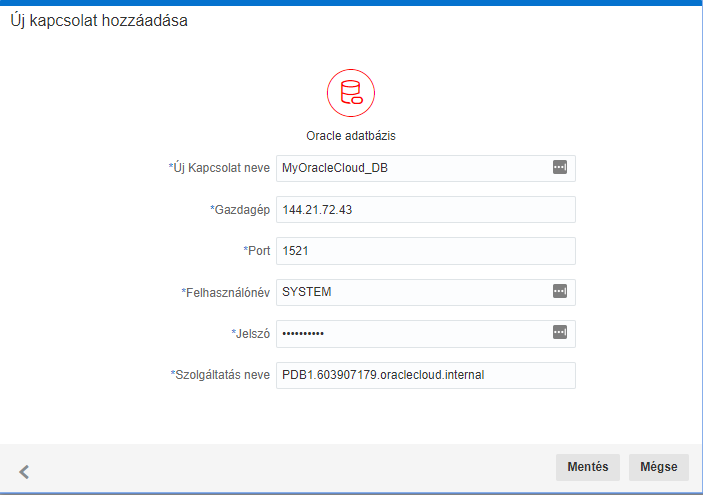
\includegraphics[width=0.9\linewidth,height=0.45\linewidth]{bence_imgs/add_connection_oracleclouddb}
	\caption{Új Oracle Cloud-beli Oracle kapcsolat hozzáadása}
	\label{fig:addconnectionoracleclouddb}
\end{figure}
Az adatbázishoz hozzákapcsolódtam SQL Developer klienst használva, és létrehoztam két teszttáblát \textit{AIRLINE} és \textit{AIRPORT} névvel, melyeket tesztadatokkal feltöltöttem. Ezt követően szerettem volna ezeket a táblákat adatforrásként használni, melyre importáláskor egy SQL lekérdezést készítek el ezáltal szűrve az adatokat. Amikor az adatforrást hozzá szerettem volna adni, nem jelentek meg az elérhető táblák között. Az elérhető táblák közt szerepelt \textit{HELP} nevű tábla, melyet próbaként töröltem az adatbázisból, de hiába kattintottam az adatok frissítésére, a tábla továbbra is ott maradt. 
\newpage\begin{figure}[h!]
	\centering
	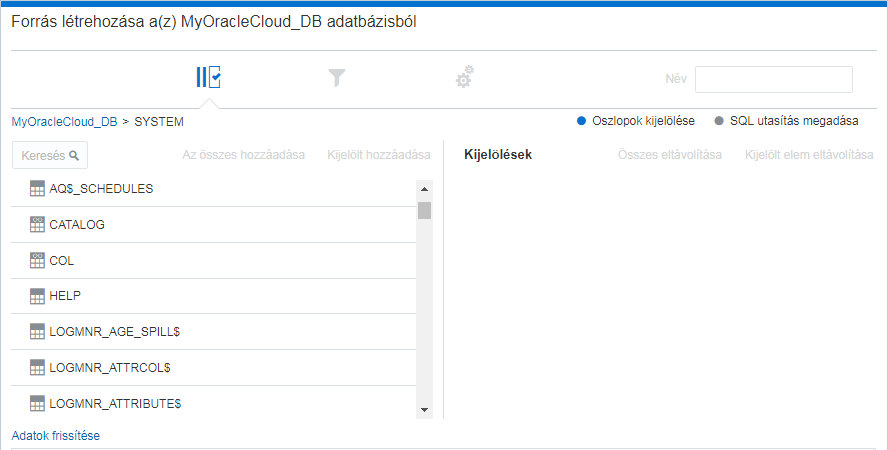
\includegraphics[width=0.7\linewidth]{bence_imgs/add_datasource_fromdb}
	\caption{Elérhető táblák listája}
	\label{fig:adddatasourcefromdb}
\end{figure}
A \ref{fig:adddatasourcefromdb}. ábrán látható az elérhető táblák listája. A listában a \textit{HELP} tábla a törlést követően frissítés ellenére is megjelenik, valamint a létrehozott teszt táblák továbbra sem elérhetőek. Összefoglalva tehát a SYSTEM user alatt csak konstans táblákat láttam, melyek létrehozás/törlés műveletekre nem reagáltak, frissítés ellenében sem. Megpróbáltam azt is, hogy újra létrehozom a kapcsolatot, de ugyanazt a konstans listát látom a SYSTEM user alatt a táblák tekintetében azesetben is.
\subsection{Amazon Web Services Oracle adatbázis}
Ezen alfejezet célja az Oracle adatbázishoz való csatlakozás tesztelése Amazon Web Services-en létrehozott Oracle adatbázis segítségével.. A kivitelezéshez létrehoztam az AWS RDS szolgáltatásával egy Oracle adatbázist futtató instancet. Az adatbázis Oracle Standard Edition 11.2.0.4.v16 verziójú, és publikus végponttal rendelkezik, helyileg Frankfurt régióban.

\begin{figure}[h!]
	\centering
	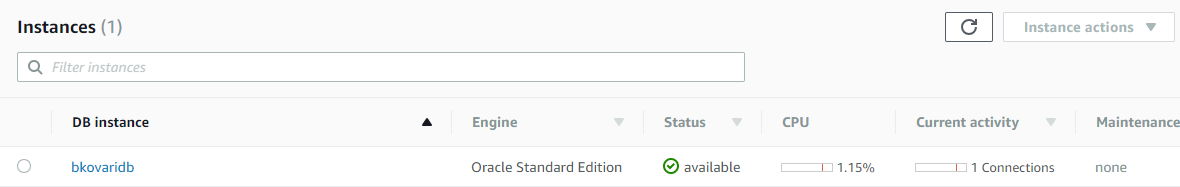
\includegraphics[width=1\linewidth,height=0.2\linewidth]{bence_imgs/oracle_db}
	\caption{Oracle Standard Edition instance}
	\label{fig:oracledb}
\end{figure}
Az adatbázishoz először SQL Developer klienst használva csatlakoztam, hogy ellenőrizzem az elérhetőséget. Csatlakozáskor a megfelelő SID-t használva (ORCL) léptem be az adatbázisba. Mivel a Visualization Tool csatlakozáskor nem SID-t használ, ezért egy \textit{show parameters service name} lekérdezést futtattva lekérdeztem az adatbázisom Service Name-t, mely ORCL\_A nevet viseli. \\ Ezt követően megkíséreltem az adatforrást hozzáadni a Visualization Tool-ban "Új kapcsolatot" létrehozásával, Oracle adatbázist kiválasztva.
\begin{figure}[h!]
	\centering
	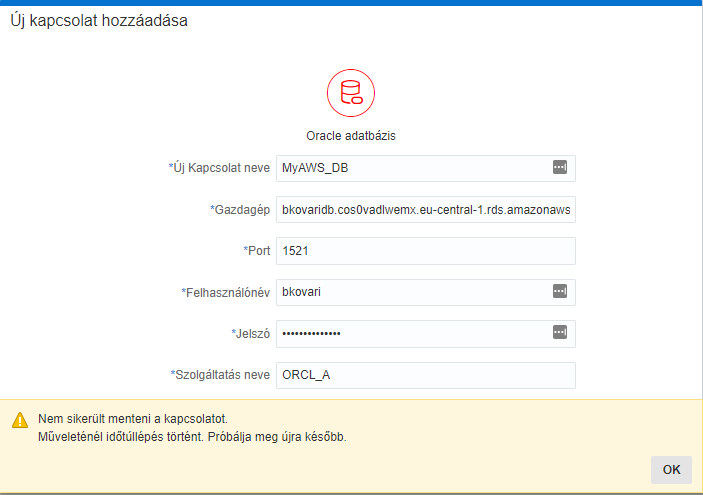
\includegraphics[width=0.9\linewidth,height=0.45\linewidth]{bence_imgs/add_connection_aws}
	\caption{Új AWS-beli Oracle kapcsolat hozzáadása}
	\label{fig:addconnectionaws}
\end{figure}
A csatlakozáshoz megadtam a megfelelő adatokat, viszont időtúllépés hiányában a kapcsolat nem jött létre. SQL Developerrel SID használata helyett ORCL\_A Service Name segítségével a csatlakozás viszont sikeres volt. Megpróbáltam még Oracle Enterprise Edition 12.1.0.2.v12 verziójú adatbázissal is, de ugyanezt tapasztaltam. Konkrét információt erre vonatkozólag nem találtam, viszont ebből arra következtetek, hogy csak az Oracle Cloudban létrehozott Oracle adatbázissal képes az a Visualization Tool kommunikálni.

\newpage
\section{Összefoglalás}
Az Oracle Visualization Tool melyet lehetőségünk volt tesztelni alapjában véve egy sokrétű és fejlett eszköz benyomását kelti. A tesztelés során a cél az eszköz általános működésének demonstrálása tesztadatokkal, a kulcsfontosságú funkciók kipróbálása, illetve az eszköz határainak beazonosítása volt. A tapasztalatok alapján hasznos funkciónak bizonyult a táblák on-the-fly módosítása új oszlop beszúrásával, saját számítások elkészítése, SQL lekérdezés megírásának lehetősége adatimportálás során, a részletesebb adatmegjelenítés (drill), valamint a széles diagramválaszték a vizualizáció tekintetében. Az eszköz ereje viszont abban rejlik, hogy mindezt online felületen tehetjük meg, bárhonnan. A dokumentációt tanulmányozva számos plusz funkciót is találtunk a Visualization Tool (vélhetően Enterprise/Data Lake edition) palettáján, mint például az integráció Big Data Toolokkal, melyekre az általunk tesztelt szolgáltatáspéldány nem képes. Illetve emellett jelentős korláttal találkoztunk egy tábla méretére vonatkozóan, vélhetően a szolgáltatáshoz előre beállított erőforráslimit végett (OCPu). Az általunk tesztelt példány ezen keretek közt oktatási célokra alkalmas: a vizualizációs technikák elsajátítására, elemzési alapok és SQL nyelv használata végett. Több erőforrással viszont nagyobb projektekre, való életbeli alkalmazások, vizualizációk elkészítésére is szívesen használnánk. Köszönjük a lehetőséget hogy részt vehettünk a Visualization Tool oktatási tréningjén, illetve megismerhettünk egy új hasznos eszközt!